\documentclass{jhwhw}
	\usepackage{enumitem}
	\usepackage{soul}
	\usepackage{float}
	
	\title{EE 4341 Homework 3}
    \author{Alex Biedny}
    \date{\today}
    \chead{EE 4341 Homework 3}
    \lhead{Alex Biedny}
    
\usepackage{graphicx}
\begin{document}

\maketitle

\problem{}
\begin{enumerate}
\item SYSCLK = 10MHz * (1/2) * 16 * (1/4) = 20MHz
PBCLK = 20MHz
\item SYSCLK = 8MHz * (1/2) * 16 * (1/2) = 32MHz
PBCLK = 16MHz
\item SYSCLK = 10MHz
PBCLK = 10MHz
\end{enumerate}

\problem{}
\begin{enumerate}
\item The flow of the function depends on a global buffer U2STAbits.UTXBF. It is possible for an interrupt to hit right after the while(U2STAbits.UTXBF) line passes, and the interrupt may change the value of U2STAbits.UTXBF.
\item The middle two lines of the function are critical, as they contain the check if the transmit buffer is full, and then the loading of the transmit buffer which can only occur after this check. If interrupts were disabled for the critical section then it would guarantee that the buffer full check is accurate when the buffer is loaded.
\item \begin{verbatim}
uint16_t SEMAPHORE1 = 1, SEMAPHORE2 = 0;

//Thread 1
wait(SEMAPHORE2);
put_out(data);
signal(SEMAPHORE1);

//Thread 2
wait(SEMAPHORE1);
put_out(data);
signal(SEMAPHORE2);
\end{verbatim}
\item \begin{verbatim}
uint16_t SEMAPHORE1 = 1, SEMAPHORE2 = 0;
\end{verbatim}
\end{enumerate}

\problem{}
\begin{enumerate}
\item 0.84
\item 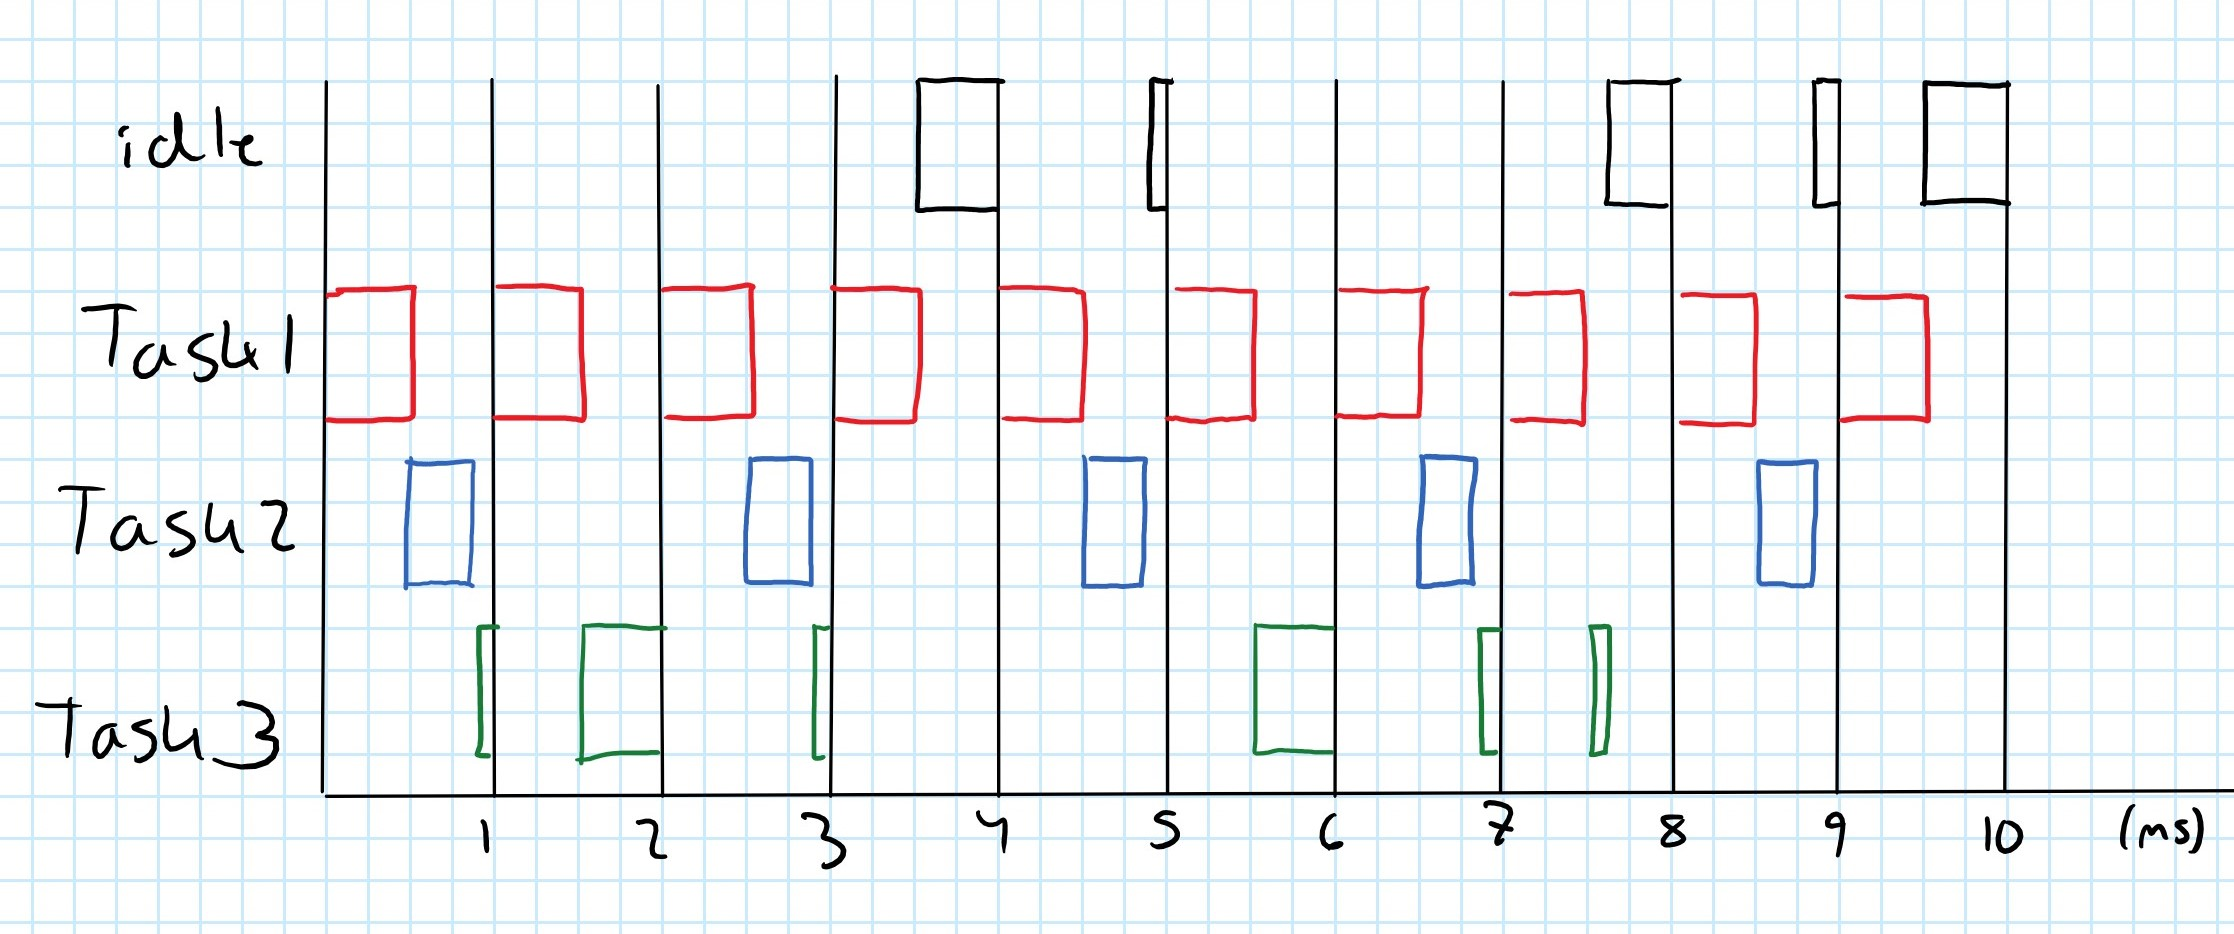
\includegraphics[scale=0.50]{HW3-1.jpg}
\item Task 1 has no latency, task 2 has 0.5ms max, and task 3 has 2.9ms max. No deadlines are missed.
\item Around 0.72ms.
\end{enumerate}

\problem{}
\begin{enumerate}
\item 1.8ms
\item 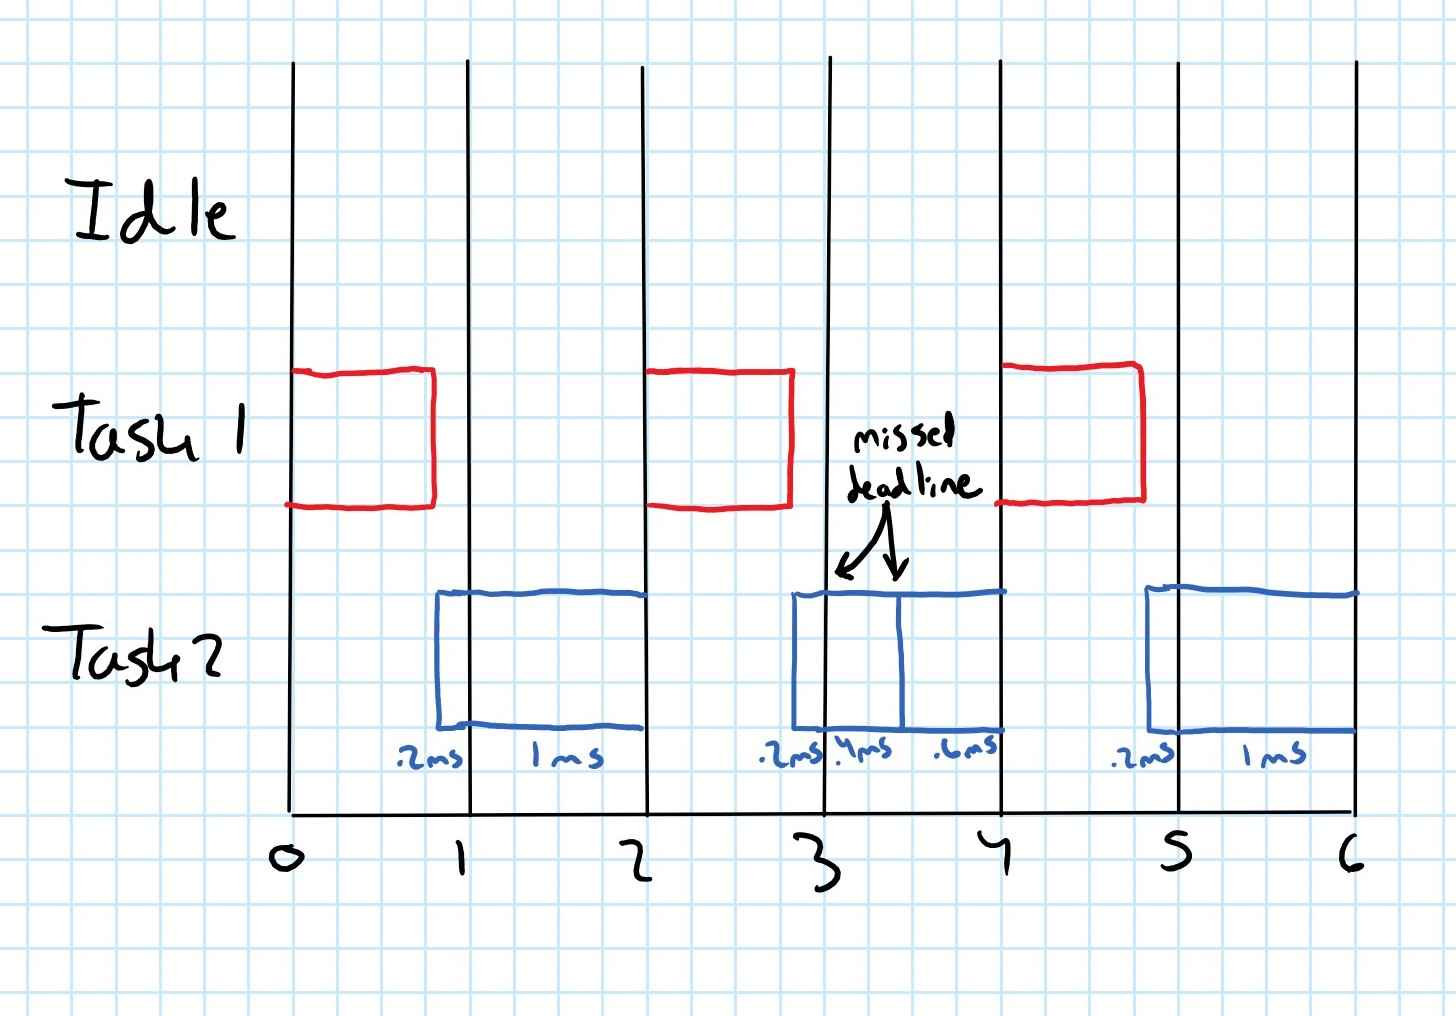
\includegraphics[scale=0.50]{HW3-2.jpg} \\
There are 5 context switches. The deadline for task 2 is missed once every hyperperiod.
\item 1.4ms
\item 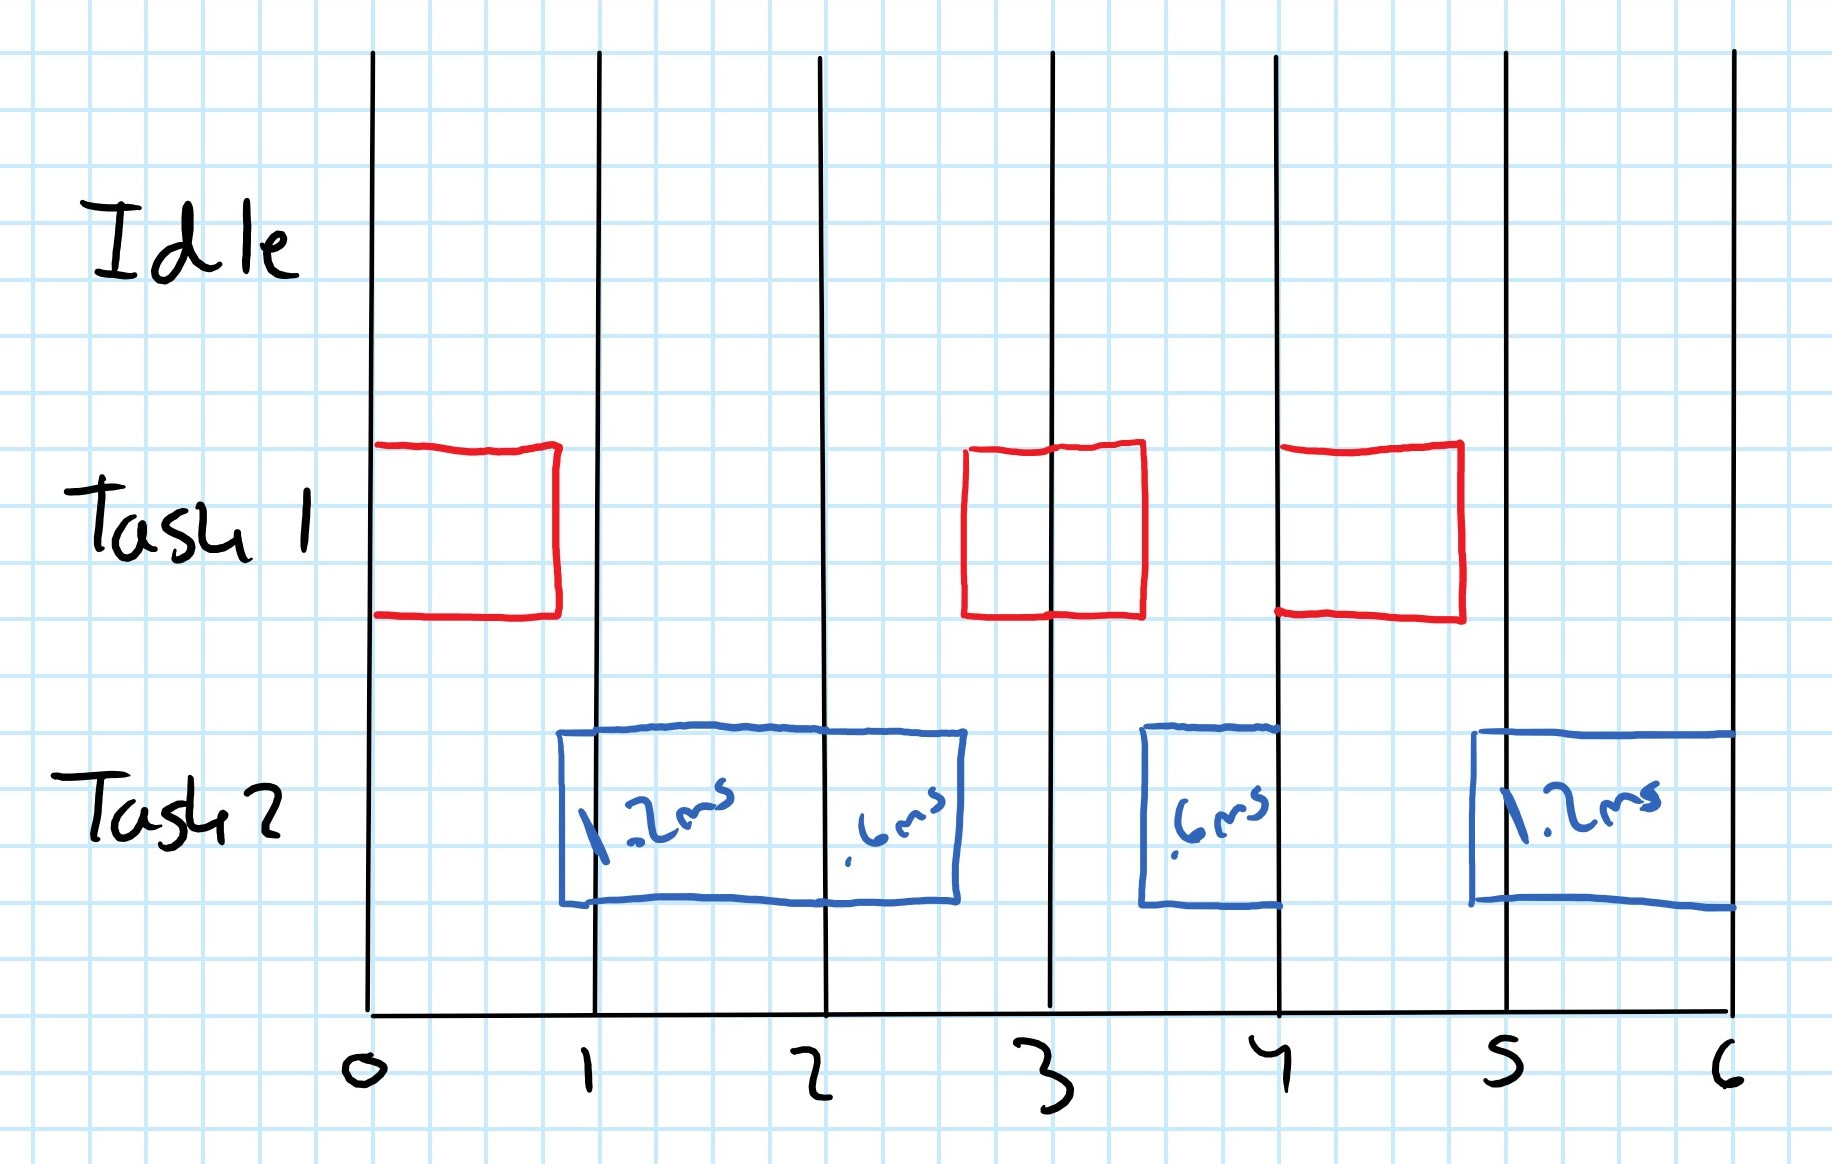
\includegraphics[scale=0.50]{HW3-3.jpg} \\
\end{enumerate}

\end{document}